\subsection{Упражнение 1}

Оцените высоты тона вокального чирпа для нескольких времён начала сегмента.

\begin{lstlisting}[language=Python]
if not os.path.exists('28042__bcjordan__voicedownbew.wav'):
    !wget https://github.com/AllenDowney/ThinkDSP/raw/master/code/28042__bcjordan__voicedownbew.wav
wave = read_wave('code_28042__bcjordan__voicedownbew.wav')
wave.normalize()
duration = 0.01
segment1 = wave.segment(start=0.1, duration=duration)
segment1.plot()
segment2 = wave.segment(start=0.2, duration=duration)
segment2.plot()
segment3 = wave.segment(start=0.3, duration=duration)
segment3.plot()
\end{lstlisting}
\begin{figure}[H]
	\begin{center}
		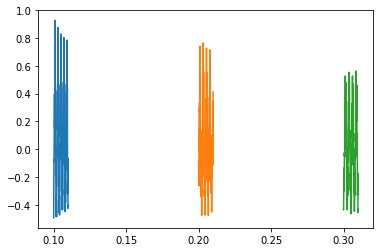
\includegraphics[scale=1]{fig/lab05/lab05_5_0.png}
		\caption{График выбранных сегментов}
	\end{center}
\end{figure}

Для определения высоты тона используем автокореляцию.

\begin{lstlisting}[language=Python]
lags1, corrs1 = autocorr(segment1)
plt.plot(lags1, corrs1, color='green')
decorate(xlabel='Lag (index)', ylabel='Correlation', ylim=[-1, 1])

lags2, corrs2 = autocorr(segment2)
plt.plot(lags2, corrs2)
decorate(xlabel='Lag (index)', ylabel='Correlation', ylim=[-1, 1])

lags3, corrs3 = autocorr(segment3)
plt.plot(lags3, corrs3, color='red')
decorate(xlabel='Lag (index)', ylabel='Correlation', ylim=[-1, 1])
\end{lstlisting}
\begin{figure}[H]
	\begin{center}
		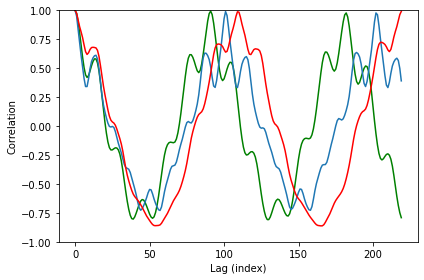
\includegraphics[scale=1]{fig/lab05/lab05_7_0.png}
		\caption{Автокорреляция сигналов}
	\end{center}
\end{figure}

Узнаем значения lag:

\begin{lstlisting}[language=Python]
low, high = 50, 200
lag1 = np.array(corrs1[low:high]).argmax() + low

low, high = 50, 200
lag2 = np.array(corrs2[low:high]).argmax() + low

low, high = 50, 200
lag3 = np.array(corrs3[low:high]).argmax() + low

lag1,lag2, lag3
\end{lstlisting}
\begin{lstlisting}
(91, 101, 109)
\end{lstlisting}

Периоды:

\begin{lstlisting}[language=Python]
period1 = lag1 / segment1.framerate
period2 = lag2 / segment2.framerate
period3 = lag3 / segment3.framerate
period1, period2, period3
\end{lstlisting}
\begin{lstlisting}
(0.0020634920634920637, 0.002290249433106576, 0.002471655328798186)
\end{lstlisting}

F max:

\begin{lstlisting}[language=Python]
frequency1 = 1 / period1
frequency2 = 1 / period2
frequency3 = 1 / period3
frequency1, frequency2, frequency3
\end{lstlisting}
\begin{lstlisting}
(484.6153846153846, 436.63366336633663, 404.5871559633028)
\end{lstlisting}

\subsection{Упражнение 2}
Инкапсулировать код автокорреляции для оценки основной частоты периодического сигнала в функцию, названную estimate\_fundamental, и исользуйте её для отслеживания высоты тона записанного звука.

Возьмём тот же звук.

\begin{lstlisting}[language=Python]
wave.make_spectrogram(2048).plot(high=4000)
\end{lstlisting}
\begin{figure}[H]
	\begin{center}
		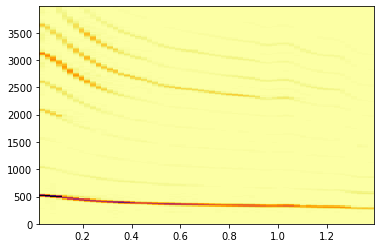
\includegraphics[scale=1]{fig/lab05/lab05_16_0.png}
		\caption{Спектрограмма записи}
	\end{center}
\end{figure}

Берём код из предыдущих пунктов и соединияем в одну функцию:

\begin{lstlisting}[language=Python]
def estimate_fundamental(segment, low=50, high=200):
  lags, corrs = autocorr(segment)
  lag = np.array(corrs[low:high]).argmax() + low
  period = lag / segment.framerate
  frequency = 1 / period
  return frequency
\end{lstlisting}

\begin{lstlisting}[language=Python]
estimate_fundamental(segment1)
\end{lstlisting}
\begin{lstlisting}
484.6153846153846
\end{lstlisting}

Чтобы сделать оценку высоты тона на всей спектрограмме надо разделить всё на маленькие сегменты и работать с ними.

\begin{lstlisting}[language=Python]
duration = wave.duration
step = 0.02
start = 0
time = []
freq = []
while start + step < duration:
  time.append(start + step/2)
  freq.append(estimate_fundamental(wave.segment(start=start,duration=step)))
  start += step
wave.make_spectrogram(2048).plot(high=900)
plt.plot(time, freq, color='blue')
decorate(xlabel='Time (s)', ylabel='Frequency (Hz)')
\end{lstlisting}
\begin{figure}[H]
	\begin{center}
		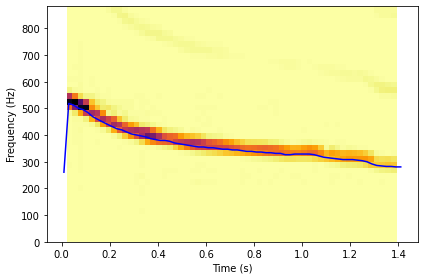
\includegraphics[scale=1]{fig/lab05/lab05_22_0.png}
		\caption{Результат}
	\end{center}
\end{figure}

\subsection{Упражнение 3}

Вычислить автокорреляцию цен в платёжной системе Bitcoin. Оценить автокореляцию и проверить на признаки переодичности процесса.

\begin{lstlisting}[language=Python]
if not os.path.exists('market-price.csv'):
    !wget https://github.com/wooftown/spbstu-telecom/raw/main/Content/market-price.csv
import pandas as pd

df = pd.read_csv('market-price.csv', parse_dates=[0])
ys = df['market-price']
ts = df.index

w = Wave(ys, framerate=1)
w.plot()

\end{lstlisting}
\begin{figure}[H]
	\begin{center}
		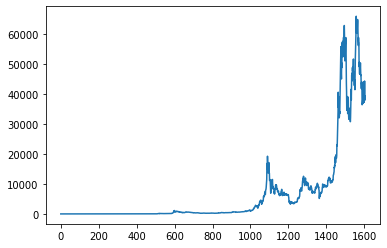
\includegraphics[scale=1]{fig/lab05/lab05_25_0.png}
		\caption{График цены на BitCoin}
	\end{center}
\end{figure}

Вычислим автокорреляцию:

\begin{lstlisting}[language=Python]
lags, corrs = autocorr(w)
plt.plot(lags, corrs)
decorate(xlabel='Lag',
         ylabel='Correlation')
\end{lstlisting}
\begin{figure}[H]
	\begin{center}
		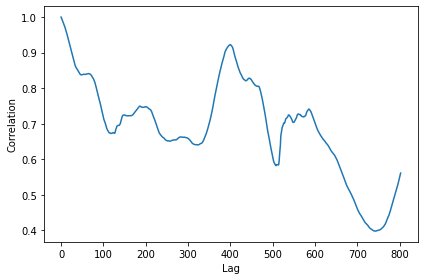
\includegraphics[scale=1]{fig/lab05/lab05_27_0.png}
		\caption{Автокорреляция функции цены на BitCoin}
	\end{center}
\end{figure}

Функция ведёт себя нестабильно, есть резкие повышения и спады. Имеется намёк на периодичность.

\subsection{Упражнение 4}

В репозитории этой книги есть блокнот Jupyter под названием saxophone.ipynb, в котором исследуются автокорреляция, восприятие высоты тона и явление, называемое подавленная основная. Прочтите этот блокнот и «погоняйте» примеры. Выберите другой сегмент записи и вновь поработайте с примерами.

\begin{lstlisting}[language=Python]
if not os.path.exists('100475__iluppai__saxophone-weep.wav'):
    !wget https://github.com/AllenDowney/ThinkDSP/raw/master/code/100475__iluppai__saxophone-weep.wav
wave = read_wave('100475__iluppai__saxophone-weep.wav')
wave.normalize()
spectrogram = wave.make_spectrogram(seg_length=1024)
spectrogram.plot(high=3000)
decorate(xlabel='Time (s)', ylabel='Frequency (Hz)')
\end{lstlisting}
\begin{figure}[H]
	\begin{center}
		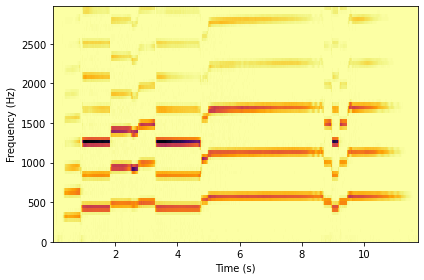
\includegraphics[scale=1]{fig/lab05/lab05_33_0.png}
		\caption{Спектрограмма звука}
	\end{center}
\end{figure}

Видна гармоническая структура во времени. Возьмём отрезок и прогоним его через все функции из блокнота.

\begin{lstlisting}[language=Python]
segment = wave.segment(start=1, duration=0.2)
segment.make_audio()
\end{lstlisting}

\begin{lstlisting}[language=Python]
spectrum = segment.make_spectrum()
spectrum.plot(high=5000)
decorate(xlabel='Frequency (Hz)', ylabel='Amplitude')
\end{lstlisting}
\begin{figure}[H]
	\begin{center}
		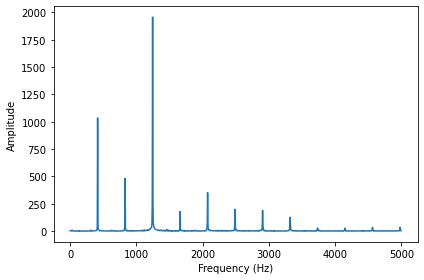
\includegraphics[scale=1]{fig/lab05/lab05_37_0.png}
		\caption{Спектр звука}
	\end{center}
\end{figure}

Спектр напомнил квадратный сигнал. Пики пришлись на 1245, 415, 830 Гц.

Далее сравним наш сегмент с треугольным сигналом с такой же низкой частотой пика.

\begin{lstlisting}[language=Python]
TriangleSignal(freq=415).make_wave(duration=0.2).make_audio()
\end{lstlisting}

У данных сигналов одинаковая воспринимаемая частота звука.

Для понимания процесса восприятия основной частоты испольщуем АКФ.

\begin{lstlisting}[language=Python]
def autocorr2(segment):
    corrs = np.correlate(segment.ys, segment.ys, mode='same')
    N = len(corrs)
    lengths = range(N, N//2, -1)

    half = corrs[N//2:].copy()
    half /= lengths
    half /= half[0]
    return half
\end{lstlisting}

\begin{lstlisting}[language=Python]
corrs = autocorr2(segment)
plt.plot(corrs[:500])
\end{lstlisting}
\begin{figure}[H]
	\begin{center}
		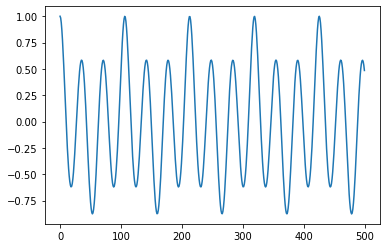
\includegraphics[scale=1]{fig/lab05/lab05_46_1.png}
		\caption{Автокорреляция}
	\end{center}
\end{figure}

Видим пик рядом с lag 100. Найдём основную частоту при помощи написанной ранее функции.

\begin{lstlisting}[language=Python]
estimate_fundamental(segment)
\end{lstlisting}

Даже если мы уберём основной тон (416 Гц), звук будет восприниматься также...

\begin{lstlisting}[language=Python]
spectrum2 = segment.make_spectrum()
spectrum2.high_pass(600)
spectrum2.plot(high=5000)
decorate(xlabel='Frequency (Hz)', ylabel='Amplitude')
\end{lstlisting}
\begin{figure}[H]
	\begin{center}
		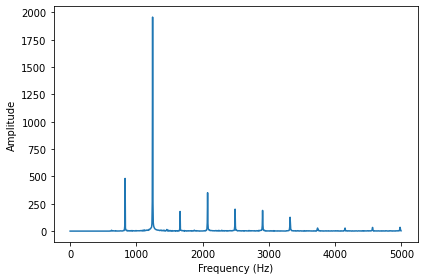
\includegraphics[scale=1]{fig/lab05/lab05_51_0.png}
		\caption{Спектр сигнала}
	\end{center}
\end{figure}

Это явление называется "missing fundamental". Для понимания, что мы слышим частоту которой нет можно снова обратиться к АКФ.

\begin{lstlisting}[language=Python]
corrs = autocorr2(segment2)
plt.plot(corrs[:500])
\end{lstlisting}
\begin{figure}[H]
	\begin{center}
		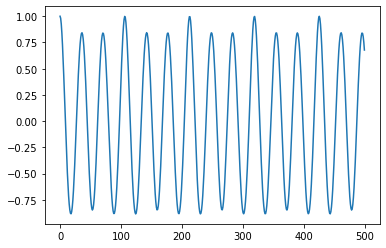
\includegraphics[scale=1]{fig/lab05/lab05_54_1.png}
		\caption{Автокорреляция}
	\end{center}
\end{figure}


Это так работает, потому что более высокие компоненты сигнала являются гармониками 416 Гц. Весь этот пример указывает нам на то, что восприятие высоты тона основано не только на спектральном анализе, но и на вычислении АКФ.

\subsection{Вывод}

В данной главе была изучена корреляция и её роль в сигналах. Также на пратике был обработан сигнал с "missing fundamental". Когда мы убирали основной тон, всё равно звук звучал также.

